%%%%%%%%%%%%%%%%%%%%%%%%%%%%%%%%%%%%%%%%%%%%%%%%%%%%%%%%%%%%%%%%%%%%%%%%%%
%
% StEvent - User Guide and Reference Manual -- LaTeX Source
%
% $Id: StEvent.tex,v 2.2 1999/11/12 18:08:33 ullrich Exp $
%
% Author: Thomas Ullrich, Nov 1999
%
%%%%%%%%%%%%%%%%%%%%%%%%%%%%%%%%%%%%%%%%%%%%%%%%%%%%%%%%%%%%%%%%%%%%%%%%%%
%
% Notes to the authors:
%
% - A template for a class reference is at the end of this file.
% - Wrap all names functions with \name{}
% - All code, examples, prototypes in \verb+ ... +\\
%   or /begin{verbatim} ... \end{verbatim}
% - Use \StEvent if you refer to the package itself (not the class)
%
% This file is best edit with xemacs and the 'Function' package loaded.
%
%%%%%%%%%%%%%%%%%%%%%%%%%%%%%%%%%%%%%%%%%%%%%%%%%%%%%%%%%%%%%%%%%%%%%%%%%%
%
% $Log
% Revision 2.33  2000/05/22 22:04:07  ullrich
% Removed StRichPixelCollection ref section and added description
% of new RICH methods to class StEvent.
%
% Revision 2.45  2000/08/23 03:14:07  ullrich
% Improved (corrected) explanation of return value
% of chi2 methods of StVertex and StTrackFitTraits.
%
% Revision 2.44  2000/08/17 00:36:31  ullrich
% Added description of StTptTrack.
%
% Revision 2.43  2000/08/17 01:18:02  ullrich
% Fixed wrong description of StZtbTriggerDetector::adc().
%
% Revision 2.42  2000/07/13 12:47:07  ullrich
% Added ZDC info provided by Clemens
%
% Revision 2.41  2000/06/29 18:00:37  ullrich
% Better description of StCtbTriggerDetector.
%
% Revision 2.40  2000/06/22 18:18:33  ullrich
% Fixed problem with page numbering. Increased textheight.
%
% Revision 2.39  2000/06/21 22:55:42  ullrich
% Added StEventInfo to ref section. Updated StEvent.
%
% Revision 2.38  2000/06/07 09:44:20  ullrich
% Modified StHit ref section.
%
% Revision 2.37  2000/06/01 21:36:17  ullrich
% Added new method flag() to StHit description.
%
% Revision 2.36  2000/06/01 16:46:23  ullrich
% Mods (add text) in StTrack and StTrackDetectorInfo.
%
% Revision 2.35  2000/05/31 14:26:26  lasiuk
% Add RICH classes and descriptions
%
% Revision 2.32  2000/05/17 17:20:01  ullrich
% Updates and improved description of StTrackTopologyMap.
% Revision 2.31  2000/05/16 13:22:39  ullrich
% More details on the second chi2 value in StTrackFitTraits.
%
% Revision 2.30  2000/05/09 11:09:30  ullrich
% Updated section on StMwcTriggerDetector and StCtbTriggerDetector.
%
% Revision 2.29  2000/04/26 21:01:44  ullrich
% Removed text for obsolete StBrowsableEvent.
%
% Revision 2.28  2000/04/20 13:31:25  ullrich
% Added description of changes to StTrackDetectorInfo.
%
% Revision 2.27  2000/04/10 19:59:34  genevb
% StRoot/StEvent/doc/tex/
%
% Revision 2.26  2000/03/30 16:55:38  ullrich
% Modified reference section for StTrack::key().
%
% Revision 2.25  2000/03/29 16:55:48  ullrich
% Added reference section and emprt user guide page for StL3Trigger.
%
% Revision 2.24  2000/03/23 18:30:50  ullrich
% Added new EMC classes to reference section.
%
% Revision 2.23  2000/03/08 14:27:45  ullrich
% Added description of new method of StVertex.
%
% Revision 2.22  2000/03/02 12:40:40  ullrich
% Added description of modified StTpcDedxPidAlgorithm
%
% Revision 2.21  2000/02/28 19:37:26  ullrich
% Added the hypperref package to add bookmarks and hyperlinks
% tp pdf documents.
%
% Revision 2.20  2000/02/24 13:25:12  ullrich
% Added RICH and EMC to the reference section. Created
% (empty) section for EMC and RICH in User Guide.
% Revision 2.19  2000/02/17 18:16:18  ullrich
% Add documentation of new SVT hit storage layout.
%
% Revision 2.18  2000/02/11 16:23:45  ullrich
% Add info on order in which primary vertices are stored
% and added description of StPrimaryVertex::flag().
  {\LARGE $ $Revision: 2.2 $ $}  \\[5mm] % replaced by cvs with current revision
  {\LARGE $ $Date: 1999/11/12 18:08:33 $ $}  % replaced by cvs with current revision
% Added Helens description of iflag (see StTrack::flag()).
%
% Revision 2.16  2000/01/27 18:38:30  ullrich
% Fixed typo in units for curvature.
%
% Revision 2.15  2000/01/12 10:45:31  ullrich
% Fixed error (underscore in text).
%
% Revision 2.14  2000/01/11 16:31:56  ullrich
% Regular update.
%
%%%%%%%%%%%%%%%%%%%%%%%%%%%%%%%%%%%%%%%%%%%%%%%%%%%%%%%%%%%%%%%%%%%%%%%%%%
\documentclass[twoside]{article}

\parindent 0pt
\parskip 6pt
\advance\textheight by 80pt%
\advance\textwidth by 80pt%
\advance\evensidemargin by -80pt%

\usepackage{graphicx}
\usepackage{psboxit}
\usepackage{amsmath}
\usepackage{amssymb}
\usepackage{amsfonts}
\usepackage{fancyhdr}
\usepackage{times}
\usepackage{verbatim}
\usepackage{makeidx}
\usepackage[dvips=true,hyperindex=true,colorlinks=true,linkcolor=blue,bookmarks=true]{hyperref}

\PScommands      % init boxit
\makeindex

%%%%%%%%%%%%%%%%%%%%%%%%%%%%%%%%%%%%%%%%%%%%%%%%%%%%%%%%%%%%%%%%%%%%
%
% Define header and footer style
  {\LARGE $ $Revision: 2.2 $ $}  \\[5mm] % replaced by cvs with current revision
  {\LARGE $ $Date: 1999/11/12 18:08:33 $ $}  % replaced by cvs with current revision
\pagestyle{fancyplain}
\rhead[\fancyplain{}{\bfseries\leftmark}]
      {\fancyplain{}{\bfseries\rightmark}}
\lhead[\fancyplain{}{\bfseries\rightmark}]
      {\fancyplain{}{\bfseries\leftmark}}
\rfoot[{}]{\fancyplain{}{\bfseries\thepage}}
\lfoot[\fancyplain{}{\bfseries\thepage}]{}
\cfoot{}

%%%%%%%%%%%%%%%%%%%%%%%%%%%%%%%%%%%%%%%%%%%%%%%%%%%%%%%%%%%%%%%%%%%%
%
% Typographic Conventions
%
%%%%%%%%%%%%%%%%%%%%%%%%%%%%%%%%%%%%%%%%%%%%%%%%%%%%%%%%%%%%%%%%%%%%
\newcommand{\name}[1]{\textsl{#1}}%  class-, function-, package names
\newcommand{\StEvent}{\textsf{StEvent}}

%%%%%%%%%%%%%%%%%%%%%%%%%%%%%%%%%%%%%%%%%%%%%%%%%%%%%%%%%%%%%%%%%%%%
%
% Define multiline labels for class reference
%
%%%%%%%%%%%%%%%%%%%%%%%%%%%%%%%%%%%%%%%%%%%%%%%%%%%%%%%%%%%%%%%%%%%%
\newcommand{\entrylabel}[1]{\mbox{\textbf{{#1}}}\hfil}%
  {\LARGE $ $Revision: 2.2 $ $}  \\[5mm] % replaced by cvs with current revision
  {\LARGE $ $Date: 1999/11/12 18:08:33 $ $}  % replaced by cvs with current revision
    {\renewcommand{\makelabel}{\entrylabel}%
     \setlength{\labelwidth}{90pt}%
     \setlength{\leftmargin}{\labelwidth}
     \advance\leftmargin by \labelsep%
      }%
    }%
  {\end{list}}
  {\LARGE $ $Revision: 2.2 $ $}  \\[5mm] % replaced by cvs with current revision
  {\LARGE $ $Date: 1999/11/12 18:08:33 $ $}  % replaced by cvs with current revision
\index{header files}
\index{StEventTypes.h file}
    {\parbox[t]{\labelwidth}{\hspace{0pt}\textbf{{#1}}}}}}
\newenvironment{Entry}%
{\renewcommand{\entrylabel}{\Entrylabel}\begin{entry}}%
where-ever possible forward declarations were used.  This is
especially true for the StEvent class itself and it is therefore
\emph{not} sufficient to include \texttt{StEvent.h} only.  Many more
header files would have to be included. This is very good for the
developers since turnaround times are minimized but obviously bad for
the users for it would be very cumbersome to each time figure out
which header files one might need and which not. Therefore are
\emph{all} header files needed to use every little bit of \StEvent\ 
put together in one single file: \texttt{StEventTypes.h}.  The
disadvantage of this approach is that every time one \StEvent\ class
changes you have to recompile all your code, even if the changed class
is not used. This, however, should not happen too often and it by far
more convenient to deal with on header file only.
  {\Large\bf STAR Offline Library Long Writeup}
To summarize: All you need when using StEvent is to include
  \mbox{\includegraphics[width=\textwidth]{StEventTitle.eps}}
  \hfill\mbox{}\\[3cm]
  {\LARGE User Guide and Reference Manual \\[5mm] for Version 2}\\[2cm]
  {\LARGE $ $Revision: 2.2 $ $}  \\[5mm] % replaced by cvs with current revision
\index{enumerations}
\index{constants}
\index{StDetectorId.h file}
\index{StVertexId.h file}
\index{StEnumerations.h file}

\StEvent\ uses a lot of enumeration for all types of purposes. This
is much more type-safe then using simple integer numbers and makes the
code much more readable. All enumerations used in \StEvent\ are defined
in \texttt{StEnumerations.h}. 
For users convenience also the ``standard'' header files
\texttt{StDetectorId.h} and  \texttt{StVertexId.h} are included therein.
%    Table of content
%
%%%%%%%%%%%%%%%%%%%%%%%%%%%%%%%%%%%%%%%%%%%%%%%%%%%%%%%%%%%%%%%%%%%%
\tableofcontents
\cleardoublepage

To remind you of the names and save you the time looking them up
all are listed below:
%    Introduction
%
%%%%%%%%%%%%%%%%%%%%%%%%%%%%%%%%%%%%%%%%%%%%%%%%%%%%%%%%%%%%%%%%%%%%


\StEvent\ version 2. Like the new version of \StEvent\ this
with revision number 1.xx. All code and documentation for the new

In this document more emphasis is put on the User Guide while the
Reference Manual part is kept shorter in terms of description of
usage.  As \StEvent\ changes this document will change accordingly and
you should always check that the revision number of the document
matches the one in the repository.

Version 2 of \StEvent\ contains significant changes as compared to the
previous versions. Part of the changes were made to cope with the
modification of the DST format in Fall of 1999, others were made to
overcome shortcomings in the previous implementation. This version is
\pagenumbering{arabic}
also more flexible in terms of extendibility to allow future track and
vertex models to be incorporated easily.  The current implementation
is also meant to be used further upstream of the analysis, i.e. in the
reconstruction phase.  As a consequence the model itself became
slightly more complex in terms of navigation and structuring.

In order to explain the model in practical terms many diagrams and
plots were included in this document. Some of them show class diagrams
using the Unified Modelling Language UML. A brief introduction to UML
is given in Appendix~\ref{sec:introUML}.\index{UML}
\begin{figure}[hb]
    \begin{center}
        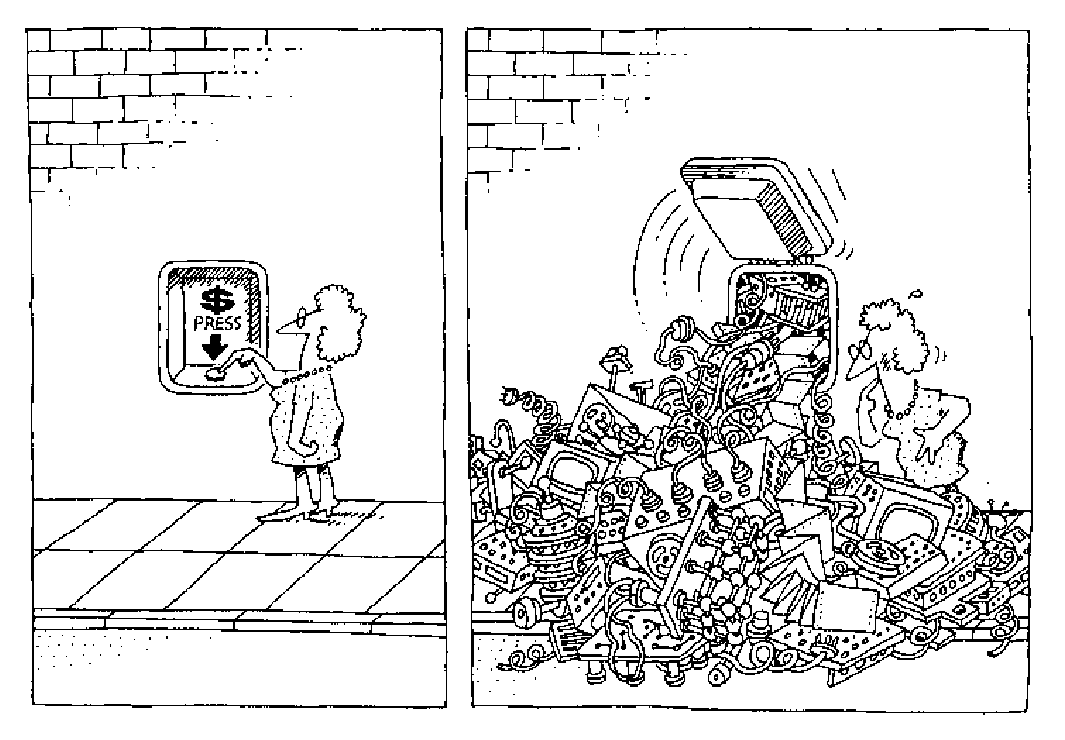
\includegraphics[width=0.9\textwidth]{cartoon1.eps}
            engineer the illusion of simplicity.}
    \end{center}
\end{figure}

\clearpage

\emph{all} header files which are needed to use every little bit of
\StEvent\ contained in one single header file named
\texttt{StEventTypes.h}.  The disadvantage of this approach is that
are used as an argument types. The strong C++ type
checking rules ensures the proper use of the enumeration
constants already during compilation.

Another important set of constants should be mentioned here as well, namely
the physical constants as defined in \texttt{PhysicalConstants.h}.
There are too many to be listed here but you should make yourself familiar
with what is available. You will find it in the \name{StarClassLibrary}
(see Sec.~\ref{sec:furtherDoc}). \index{StarClassLibrary}
In order to define the units of the various physical constants another set
of constants defined in \texttt{SystemOfUnits.h} is used (also from 
\name{StarClassLibrary}). The latter is described in section \ref{sec:units}.
\StEvent\ uses a lot of enumerations for all types of purposes. This
is much more type-safe then using simple integer numbers and makes the
code more readable. All enumerations used in \StEvent\ are defined in
\texttt{StEnumerations.h}.  For users convenience some non-\StEvent\
header files as \texttt{StDetectorId.h}, \texttt{StVertexId.h} and
\subsubsection{Numbering Scheme}
All numbering follows \emph{strictly} the C/C++ convention. This
includes not only indices as usual but also for example sector
numbers, row numbers and wafer numbers. If you follow this rule things
become less confusing for there is only one way of counting. This
allows to follow the usual C/C++ syntax in all forms:
\begin{verbatim}
const int nSectors = 24;
for (int i=0; i<nSectors; i++)
    // ...
\end{verbatim}
If you find a deviation from this rule it is a bug.
                             kEndcapEmcPreShowerId,
                             kEndcapSmdEtaStripId,
\index{references}
\index{pointers}
                             kZdcWestId,
Many methods (or member functions) or \StEvent\ classes return
objects by \emph{reference} or by \emph{pointer}. This is sometimes confusing
but there is a idea behind this. Whenever an object is returned
by reference it is guaranteed to exist. No questions asked. If the
object is a container it might be empty, i.e. it has zero size,
but you ask for it you get it. Objects returned by pointer, however,
are \emph{not} guaranteed to exist. You might get a NULL pointer back.
It is always a good idea to check if you really get what you asked
for. Dereferencing a NULL pointer can be painful.

                             kOtherVtxId};

enum StDedxMethod           {kUndefinedMethodId,
\index{units}
\index{system of units}
All physics quantities in \StEvent\ are stored using the official STAR
units: cm, GeV and Tesla.  Angles are given in radians\footnote{Note,
    that here \StEvent\ deviates from STAR guidelines where degrees
    are declared the official units.}  In order to maintain a coherent
system of units it is recommended to use the definitions in
\texttt{SystemOfUnits.h} from the StarClassLibrary. They allow to
'assign' a unit to a given variable by multiplying it with a constant
named accordingly (centimeter, millimeter, kilometer, tesla, MeV,
...).  The value of the constants is thus that the result after the
multiplication follows always the STAR system of units.

                             tpcOther,
                             ftpcConformal,
                             svtTpcSvm,
                             svtTpcEst,
                             svtTpcPattern};

enum StRichPidFlag          {eNoMip,
                             eFastEnough,
                             eLightOnPadPlane};
\end{verbatim}

Note that often the enumeration type names (e.g. \texttt{StTrackType})
are used as argument types. The strong C++ type checking rules ensures
the proper use of the enumeration constants already during
compilation.

Another important set of constants should be mentioned here as well,
namely the physical constants defined in \texttt{PhysicalConstants.h}.
There are too many to be listed here but you should make yourself
familiar with what constants are available. You will find the header
file in the \name{StarClassLibrary} (see Sec.~\ref{sec:furtherDoc}).
\index{StarClassLibrary} In order to define the units of the various
physical constants another set of constants defined in
\texttt{SystemOfUnits.h} is used (also from \name{StarClassLibrary}).
The latter is described in section \ref{sec:units}.

\subsection{Conventions}
\index{conventions}
\label{sec:conventions}

\subsubsection{Numbering Scheme}
\label{sec:conventionsNumbering}

All numbering follows \emph{strictly} the C/C++ convention, i.e. the
first element in an array has the index 0. This is valid for all
container, collections and lists. Here it is important to remember
that many (but not all) official STAR numbering schemes start counting
at 1.  Examples are TPC sectors and padrows, SVT barrels, layers, ladders and
wafers. Do not forget to subtract 1 when using this scheme for
addressing elements in a container.

TPC, SVT and FTPC hits return their hardware address in STAR units.
In order to select the hit container in which a hit \texttt{h} is
stored you must write:
Further documentation can be found in the StarClassLibrary manual
(see Sec.~\ref{sec:furtherDoc}).\vfill
\end{verbatim}

programming language and C/C++ played only a minor role. Again, the only
\index{ROOT}
\index{persistence}
All \StEvent\ classes inherit from \texttt{StObject} which itself inherits
from \texttt{TObject}. During the build of \StEvent\ all classes run through
\texttt{rootcint}. This adds the following features:
\item \texttt{StTpcHit::padrow()}
\item All \StEvent\ classes can be used on the \texttt{root4star} command line.
\item Almost all \StEvent\ classes are persistent capable, i.e. they can be stored
    in ROOT files.
\item \textrm{StSvtHit::wafer(})
As usual each coin has two sides. The disadvantage of this is that we cannot use
some features of the ANSI/ISO C++ and from the Strandard C++ Library as:
\end{itemize}
See the corresponding reference sections for more.
\item templates 
\item STL containers and algorithms    
\item namespaces    

This however applies for the header files only. Source files are not processed
via \texttt{rootcint} and therefore all the stuff mentioned above can be used.
And indeed in the implementation of various \StEvent\ classes we make heavily
use of STL features.
\begin{figure}[hbt]
for it you get it. Objects returned by pointer, however, are
\emph{not} guaranteed to exist. You might get a \texttt{NULL} pointer
back.  It is always a good idea to check if you really get what you
asked for.  Dereferencing a \texttt{NULL} pointer can be painful.

As you will see in the reference section many methods are provided in
two versions: a constant and a non-constant version. Don't worry about
cout << "STAR units:" << endl;
cout << "a = " << a << " cm" << endl;
cout << "b = " << b << " cm" << endl;
\index{container}
\index{iterators}
Version 2 of \StEvent\ comes with a new naming scheme for containers.
All containers used in \StEvent\ store objects by pointer. Technically
they are all vectors and therefore allow random-access as in
//
//   Print in personal units
//
that is they are ordered collections. There are two different types
of containers, so called structural and non-structural containers.
What that means is rather simple. Structural containers \emph{own}
the objects they contain the others not. If you delete a structural
cout << "E1 = " << E1/TeV << " TeV" << endl;
cout << "E2 = " << E2/keV << " keV" << endl;
\end{verbatim}
The resulting printout is:
\begin{verbatim}
STAR units:
a = 10 cm
b = 0.4 cm
c = 2.54 cm
E1 = 0.13 GeV
E2 = 0.1234 GeV

My units:
a = 100 mm
and non-structural collection. Their interface is the same and they
act they same. The secret lies in their implementation. If you create
a container by your own you should always use the non-structural
containers. Those you van create and delete without doing \StEvent\ 
\end{verbatim}
your back to wall with a sharp knife on your throat.
manual (see Sec.~\ref{sec:furtherDoc}).\vfill
All containers used in \StEvent\ are defined in the \texttt{StContainers.h} header
file and are based on StArray which was written by Victor Perevoztchikov.
\index{StContainers.h}
\label{sec:Persistence}
\index{ROOT} \index{persistence} All \StEvent\ classes inherit from
\texttt{StObject} which itself inherits from \texttt{TObject}. During
the build of \StEvent\ all classes run through \texttt{rootcint}. This
adds the following features:
\begin{enumerate}
\item All \StEvent\ classes can be used on the \texttt{root4star}
    command line.
\item Almost all \StEvent\ classes are persistent capable, i.e. they
    can be stored in ROOT files.
\end{enumerate}
As usual each coin has two sides. The disadvantage of this is that we
cannot use some features of the ANSI/ISO C++ and from the Standard C++
Library as:
\begin{itemize}
\item type bool
\item templates
\item STL containers and algorithms
\item namespaces
All containers are based on modified ROOT \index{ROOT} collections. They
allow to make \StEvent\ persistent. They good thing with \texttt{StArray}
is that all those containers offer an almost ANSI/ISO compatible interface.
This means that \emph{both} containers classes provide the essential methods
listed below. Replace \texttt{ClassName} with whatever \StEvent\ class.
    \begin{center}
        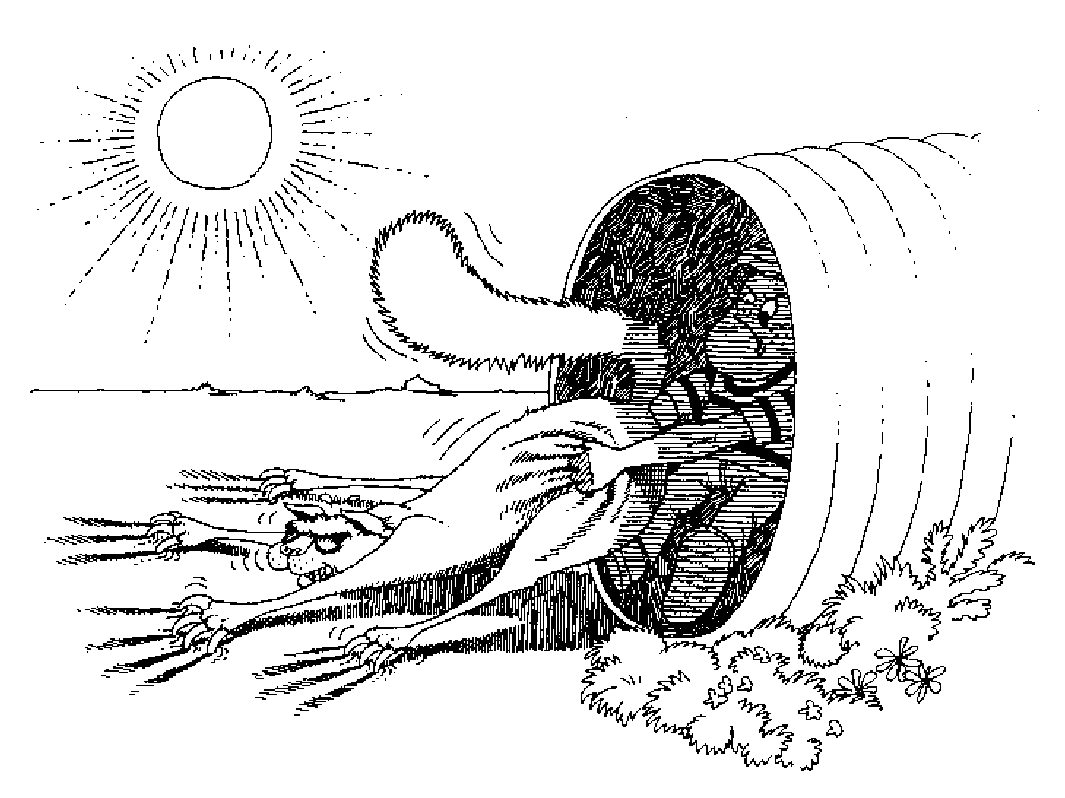
\includegraphics[width=0.5\textheight]{cartoon4.eps}
        \caption{Persistence saves the state and class of an object
            across time or space.}
    \end{center}
\end{figure}

ROOT uses typedefs for the built-in standard C++ types. This is pretty
confusing but has a good reason when it comes to persistence. This way

independent of the platform.  The ANSI/ISO standard only requires
that: \texttt{char} $\le$ \texttt{short} $\le$ \texttt{int} $\le$
    Copy constructor. Structural containers copies also the
    objects it contains.

The types used in \StEvent\ are defined as follows:
\begin{verbatim}
    Adds object pointed to by \texttt{pobj}. If the container is not large
    enough it will automatically resize.
typedef short          Short_t;     //Signed Short integer 2 bytes
typedef unsigned short UShort_t;    //Unsigned Short integer 2 bytes
    Returns the current size of the container, i.e. the number
    of stored elements.

typedef unsigned long  ULong_t;     //Unsigned long integer 4 bytes
typedef float          Float_t;     //Float 4 bytes
typedef double         Double_t;    //Float 8 bytes
typedef unsigned char  Bool_t;      //Boolean
    Deletes all elements.

code other than in the definition of class data member. Even worse
this can have disadvantages when it comes to calls to system functions
and speed. It also makes code less portable and readable.  Don't use
them only because you see them used in \StEvent.

\subsection{Container and Iterators}
\label{sec:Container}
\index{container} \index{iterators} Version 2 of \StEvent\ comes with
a new naming scheme for containers.  All containers used in \StEvent\
store objects by pointer. Technically they are all vectors and
therefore allow random-access as in
\begin{verbatim}
    pointer_to_object = container[i];
    Deletes element referred to by iterator \texttt{iter}.
    If applied to structural containers the objects gets deleted.
containers, so called structural and non-structural containers.  What
that means is rather simple. Structural containers \emph{own} the
objects they contain the others not. If you delete a structural
container all objects stored in it get deleted as well.
\begin{itemize}
\item All \textbf{s}tructural \textbf{vec}tors which store
There are many more than one can describe here.
If you want to learn more you better have a look at the
\texttt{StArray.h} source code directly.
    \textbf{p}oin\textbf{t}e\textbf{r}s carry the prefix
Needless to say that every container comes with two iterators a
constant and a non-constant version.  The name of each iterators is
composed of the name of container and the
contain and we are done. Hence a structural container which holds
objects (or better pointer to objects) of type \texttt{StTrackNode} is
iterators StSPtrVecTrackNodeIterator and
StSPtrVecTrackNodeConstIterator are defined.  Iterators care if the
iterate over about structural or non-structural containers so there
are two sets of iterators for \texttt{StSPtrVecTrackNode} and
they same. The secret lies in their implementation. If you create a
container by your own you should always use the non-structural
containers. Those you can create and delete without doing \StEvent\
any harm. Never delete a structural container unless you stand with
your back to a wall and a sharp knife on your throat.
version has some advantages and is safer.
All containers used in \StEvent\ are defined in the
\texttt{StContainers.h} header file and are based on \texttt{StArray}
which was written by Victor Perevoztchikov.  \index{StContainers.h}
Currently the following containers are in use:
\begin{verbatim}
StPtrVecHit
StPtrVecTrack
StPtrVecTrackPidTraits
StSPtrVecFtpcHit
StSPtrVecKinkVertex
StSPtrVecPrimaryTrack
StSPtrVecPrimaryVertex
StSPtrVecSvtHit
StSPtrVecTpcHit
A warning at the end. Although StArray provides a interface compatible
with the Standard C++ Library (former STL) it is not guaranteed that
the standard algorithms will work (\texttt{sort}, \texttt{accumulate},
\texttt{copy}, \texttt{find}, ...). You better check this from case to
case. Don't say you haven't been warned.

For your own analysis (or reconstruction) code you might use the standard
STL containers together with StEvent freely provided that you classes are not
processed via \texttt{rootcint}. Since STL containers are transient they
are more efficient if speed and use less memory if this is your concern.
compatible interface.  This means that \emph{both} container classes
provide the essential methods listed below. Replace \texttt{ClassName}
with any \StEvent\ class one might find in a container.
\begin{Entry}
\item[Public\\ Constructors]
    \verb+StPtrVecClassName();+\\
    \verb+StSPtrVecClassName();+\\
    Constructs an instance with zero length.

    \verb+StPtrVecClassName(UInt_t nelem);+\\
    \verb+StSPtrVecClassName(UInt_t nelem);+\\
place and at the right time.  The only two methods you should be aware
of are:
    \verb+StPtrVecClassName(const StPtrVecClassName& vec);+\\

    to structural containers the object gets also deleted.
    
    Returns a pointer to the current StEvent object.
    Returns the pointer to the \texttt{i}'th element where \texttt{i}
    runs from 0 to \texttt{size()-1}.
    Returns a pointer to the current StRun object.
    This object is only updates for a new run, else you will
    get always the same instance.

Needless to say that every container comes with two iterators, a
constant and a non-constant version.  The name of each iterator is
composed of the name of the container and the
suffix \texttt{Iterator} or \texttt{ConstIterator}.\\
Example: For the structural container \texttt{StSPtrVecTrackNode} the
iterators \texttt{StSPtrVecTrackNodeIterator} and

if they iterate over structural or non-structural containers so there
are different iterators for \texttt{StSPtrVecTrackNode} and
\texttt{StPtrVecTrackNode} containers.
    
    \verb+Bool_t  doPrintMemoryInfo;+\\
    Switch on/off checks on memory usage of \StEvent\


In order to get started it is always a good idea to study a simple
\subsection{Run Header} 
is the place to check if you don't understand the meaning of certain
    cout << "center of mass energy: " << run->centerOfMassEnergy() << endl;
can be reached directly from the \texttt{StEvent} objects.  Here's a
           << tpcMon->n_clus_tpc_in[i] << " cluster" << endl;
       // Assume it's a pion
cout << tpcDedx.traits()->mean() << endl;
     << theHits.size() << " hits" << endl;

for (int i=0; i<theHits.size(); i++) {
    cout << theHits[i]->position() << endl;
%    Reference Manuel
    assert(theHits[i]->ladder() == iladder);
    assert(theHits[i]->wafer() == iwafer);
\part{Reference Manuel}
\end{verbatim}

\subsection{Remarks on Hits and Vertices}
\index{StMeasuredPoint}
The fact that hits and vertices inherit from the same base class
\texttt{StMeasuredPoint} can be used wherever positions and errors
are what count. Take for an example a track fit. What you have to pass
to the fitting algorithm are the points and the errors. A fitter usually
gives a damn if the position was taken in the SVT or TPC. What counts
are the coordinates and their weight which depends on the errors.
\end{verbatim}
Note that some constructors are omitted, especially the ones which
take tables as arguments. They are for internal use only (even if
public).

Default constructors, destructors, assignment operators and copy
constructors are not listed.  \texttt{Inline} declarations are omitted
throughout the documentation.
\begin{figure}[hb]
    \begin{center}
        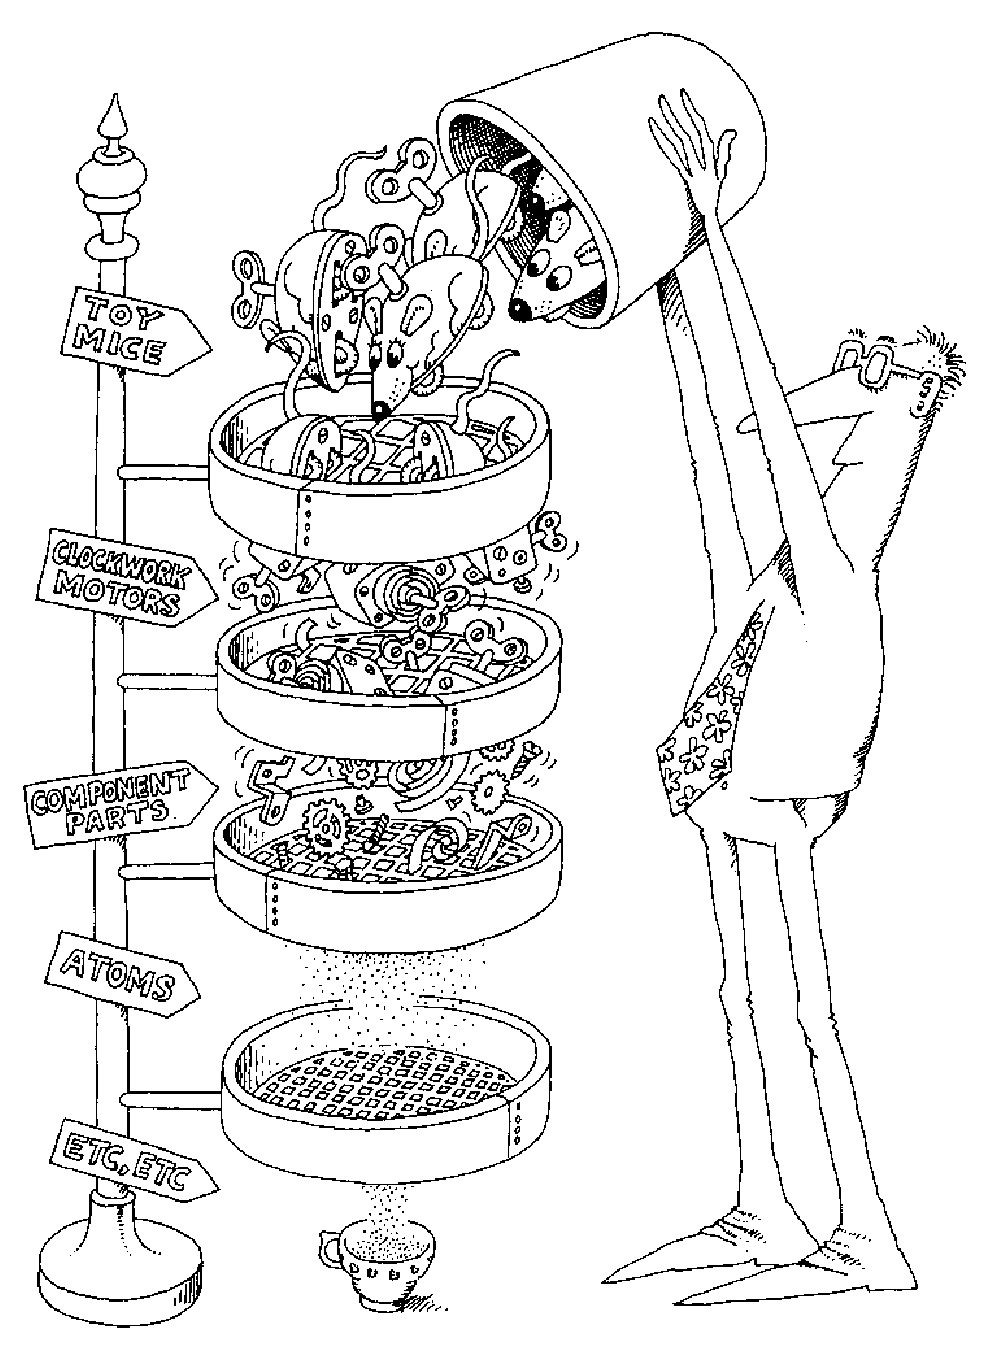
\includegraphics[width=0.45\textheight]{cartoon3.eps}
        \caption{Abstractions from a hierarchy.}
    \end{center}
\end{figure}
    \verb+#include "StTpcHitCollection.h"+\\
    \verb+class StTpcHitCollection;+\\
%\subsection{StBrowsableEvent}
%\index{StBrowsableEvent|textbf}
%\label{sec:StCtbCounter}
%\clearpage
    
%\subsection{StContainers}
%\index{StContainers|textbf}
%\label{sec:StContainers}
%\clearpage
    
%\subsection{StCtbSoftwareMonitor}
%\index{StCtbSoftwareMonitor|textbf}
%\label{sec:StCtbSoftwareMonitor}
%\clearpage
    
%\subsection{StCtbTriggerDetector}
%\index{StCtbTriggerDetector|textbf}
%\label{sec:StCtbTriggerDetector}
%\clearpage
    
%\subsection{StDedxPidTraits}
%\index{StDedxPidTraits|textbf}
%\label{sec:StDedxPidTraits}
%\clearpage
    
%\subsection{StEmcSoftwareMonitor}
%\index{StEmcSoftwareMonitor|textbf}
%\label{sec:StEmcSoftwareMonitor}
%\clearpage
    
%\subsection{StEnumerations}
%\index{StEnumerations|textbf}
%\label{sec:StEnumerations}
%\clearpage
    
%\subsection{StEvent}
%\index{StEvent|textbf}
%\label{sec:StEvent}
%\clearpage
    
%\subsection{StEventSummary}
%\index{StEventSummary|textbf}
%\label{sec:StEventSummary}
%\clearpage
    
%\subsection{StEventTypes}
%\index{StEventTypes|textbf}
%\label{sec:StEventTypes}
%\clearpage
    
%\subsection{StFtpcHit}
%\index{StFtpcHit|textbf}
%\label{sec:StFtpcHit}
%\clearpage
    
%\subsection{StFtpcHitCollection}
%\index{StFtpcHitCollection|textbf}
%\label{sec:StFtpcHitCollection}
%\clearpage
    
%\subsection{StFtpcPlaneHitCollection}
%\index{StFtpcPlaneHitCollection|textbf}
%\label{sec:StFtpcPlaneHitCollection}
%\clearpage
    
%\subsection{StFtpcSectorHitCollection}
%\index{StFtpcSectorHitCollection|textbf}
%\label{sec:StFtpcSectorHitCollection}
%\clearpage
    
%\subsection{StFtpcSoftwareMonitor}
%\index{StFtpcSoftwareMonitor|textbf}
%\label{sec:StFtpcSoftwareMonitor}
%\clearpage
    
%\subsection{StFunctional}
%\index{StFunctional|textbf}
%\label{sec:StFunctional}
%\clearpage
    
%\subsection{StGlobalSoftwareMonitor}
%\index{StGlobalSoftwareMonitor|textbf}
%\label{sec:StGlobalSoftwareMonitor}
%\clearpage
    
%\subsection{StGlobalTrack}
%\index{StGlobalTrack|textbf}
%\label{sec:StGlobalTrack}
%\clearpage
    
%\subsection{StHelixModel}
%\index{StHelixModel|textbf}
%\label{sec:StHelixModel}
%\clearpage
    
%\subsection{StHit}
%\index{StHit|textbf}
%\label{sec:StHit}
%\clearpage
    
%\subsection{StKinkVertex}
%\index{StKinkVertex|textbf}
%\label{sec:StKinkVertex}
%\clearpage
    
%\subsection{StL0Trigger}
%\index{StL0Trigger|textbf}
%\label{sec:StL0Trigger}
%\clearpage
    
%\subsection{StL3SoftwareMonitor}
%\index{StL3SoftwareMonitor|textbf}
%\label{sec:StL3SoftwareMonitor}
%\clearpage
    
%\subsection{StMeasuredPoint}
%\index{StMeasuredPoint|textbf}
%\label{sec:StMeasuredPoint}
%\clearpage
    
%\subsection{StMwcTriggerDetector}
%\index{StMwcTriggerDetector|textbf}
%\label{sec:StMwcTriggerDetector}
%\clearpage
    
%\subsection{StPrimaryTrack}
%\index{StPrimaryTrack|textbf}
%\label{sec:StPrimaryTrack}
%\clearpage
    
%\subsection{StPrimaryVertex}
%\index{StPrimaryVertex|textbf}
%\label{sec:StPrimaryVertex}
%\clearpage
    
%\subsection{StRichPixel}
%\index{StRichPixel|textbf}
%\label{sec:StRichPixel}
%\clearpage
    
%\subsection{StRichSoftwareMonitor}
%\index{StRichSoftwareMonitor|textbf}
%\label{sec:StRichSoftwareMonitor}
%\clearpage
    
%\subsection{StRun}
%\index{StRun|textbf}
%\label{sec:StRun}
%\clearpage
    
%\subsection{StRunSummary}
%\index{StRunSummary|textbf}
%\label{sec:StRunSummary}
%\clearpage
    
%\subsection{StSoftwareMonitor}
%\index{StSoftwareMonitor|textbf}
%\label{sec:StSoftwareMonitor}
%\clearpage
    
%\subsection{StSsdHit}
%\index{StSsdHit|textbf}
%\label{sec:StSsdHit}
%\clearpage
    
%\subsection{StSvtHit}
%\index{StSvtHit|textbf}
%\label{sec:StSvtHit}
%\clearpage
    
%\subsection{StSvtHitCollection}
%\index{StSvtHitCollection|textbf}
%\label{sec:StSvtHitCollection}
%\clearpage
    
%\subsection{StSvtLadderHitCollection}
%\index{StSvtLadderHitCollection|textbf}
%\label{sec:StSvtLadderHitCollection}
%\clearpage
    
%\subsection{StSvtLayerHitCollection}
%\index{StSvtLayerHitCollection|textbf}
%\label{sec:StSvtLayerHitCollection}
%\clearpage
    
%\subsection{StSvtSoftwareMonitor}
%\index{StSvtSoftwareMonitor|textbf}
%\label{sec:StSvtSoftwareMonitor}
%\clearpage
    
%\subsection{StSvtWaferHitCollection}
%\index{StSvtWaferHitCollection|textbf}
%\label{sec:StSvtWaferHitCollection}
%\clearpage
    
%\subsection{StTpcDedxPidAlgorithm}
%\index{StTpcDedxPidAlgorithm|textbf}
%\label{sec:StTpcDedxPidAlgorithm}
%\clearpage
    
%\subsection{StTpcHit}
%\index{StTpcHit|textbf}
%\label{sec:StTpcHit}
%\clearpage
    
%\subsection{StTpcHitCollection}
%\index{StTpcHitCollection|textbf}
%\label{sec:StTpcHitCollection}
%\clearpage
    
%\subsection{StTpcPadrowHitCollection}
%\index{StTpcPadrowHitCollection|textbf}
%\label{sec:StTpcPadrowHitCollection}
%\clearpage
    
%\subsection{StTpcPixel}
%\index{StTpcPixel|textbf}
%\label{sec:StTpcPixel}
%\clearpage
    
%\subsection{StTpcSectorHitCollection}
%\index{StTpcSectorHitCollection|textbf}
%\label{sec:StTpcSectorHitCollection}
%\clearpage
    
%\subsection{StTpcSoftwareMonitor}
%\index{StTpcSoftwareMonitor|textbf}
%\label{sec:StTpcSoftwareMonitor}
%\clearpage
        
%\subsection{StTrack}
%\index{StTrack|textbf}
%\label{sec:StTrack}
%\clearpage
    
%\subsection{StTrackDetectorInfo}
%\index{StTrackDetectorInfo|textbf}
%\label{sec:StTrackDetectorInfo}
%\clearpage
    
%\subsection{StTrackFitTraits}
%\index{StTrackFitTraits|textbf}
%\label{sec:StTrackFitTraits}
%\clearpage
    
%\subsection{StTrackGeometry}
%\index{StTrackGeometry|textbf}
%\label{sec:StTrackGeometry}
%\clearpage
    
%\subsection{StTrackNode}
%\index{StTrackNode|textbf}
%\label{sec:StTrackNode}
%\clearpage
    
%\subsection{StTrackPidTraits}
%\index{StTrackPidTraits|textbf}
%\label{sec:StTrackPidTraits}
%\clearpage
    
%\subsection{StTrackTopologyMap}
%\index{StTrackTopologyMap|textbf}
%\label{sec:StTrackTopologyMap}
%\clearpage
    
%\subsection{StTrigger}
%\index{StTrigger|textbf}
%\label{sec:StTrigger}
%\clearpage
    
%\subsection{StTriggerDetectorCollection}
%\index{StTriggerDetectorCollection|textbf}
%\label{sec:StTriggerDetectorCollection}
%\clearpage
    
%\subsection{StV0Vertex}
%\index{StV0Vertex|textbf}
%\label{sec:StV0Vertex}
%\clearpage
    
%\subsection{StVertex}
%\index{StVertex|textbf}
%\label{sec:StVertex}
%\clearpage
    
%\subsection{StVpdTriggerDetector}
%\index{StVpdTriggerDetector|textbf}
%\label{sec:StVpdTriggerDetector}
%\clearpage
    
%\subsection{StXiVertex}
%\index{StXiVertex|textbf}
%\label{sec:StXiVertex}
%\clearpage
    
%\subsection{StZdcTriggerDetector}
%\index{StZdcTriggerDetector|textbf}
%\label{sec:StZdcTriggerDetector}
%\clearpage
\begin{Entry}
    \verb+Int_t operator!=(const StVertex&) const;+\\
\end{Entry}
\clearpage


\subsection{StVpdTriggerDetector}
\appendix
\label{sec:StVpdTriggerDetector}
\begin{Entry}
\item[Summary]
\item[Synopsis]
    \verb+#include "StVpdTriggerDetector.h"+\\
UNL stands for Unified Modelling Language. It is the current standard
\item[Description]
\item[Related Classes]
\item[Public\\ Constructors]
    \verb+StVpdTriggerDetector();+\\
    \verb+StVpdTriggerDetector(const dst_TrgDet_st&);+\\
\item[Public Member\\ Functions]
    \verb+UInt_t numberOfVpdCounters() const;+\\
    \verb+Float_t adc(UInt_t) const;+\\
    \verb+Float_t time(UInt_t) const;+\\
    \verb+Float_t minimumTime(StBeamDirection) const;+\\
    \verb+Float_t vertexZ() const;+\\
    \verb+void setAdc(UInt_t, Float_t);+\\
    \verb+void setTime(UInt_t, Float_t);+\\
    \verb+void setMinimumTime(StBeamDirection, Float_t);+\\
    \verb+void setVertexZ(Float_t);+\\
\end{Entry}
\clearpage


\subsection{StXiVertex}
\index{StXiVertex|textbf}
\label{sec:StXiVertex}
\begin{Entry}
\item[Summary]
\item[Synopsis]
    \verb+#include "StXiVertex.h"+\\
    \verb+class StXiVertex;+\\
\item[Description]
\item[Related Classes]
\item[Public\\ Constructors]
    \verb+StXiVertex();+\\
    \verb+StXiVertex(const dst_vertex_st&, const dst_xi_vertex_st&);+\\
\item[Public Member\\ Functions]
    \verb+StVertexId type() const;+\\
    \verb+UInt_t numberOfDaughters() const;+\\
    \verb+StTrack* daughter(UInt_t = 0);+\\
    \verb+const StTrack* daughter(UInt_t = 0) const;+\\
    \verb+StPtrVecTrack daughters(StTrackFilter&);+\\
    \verb+Float_t dcaBachelorToPrimaryVertex() const;+\\
    \verb+Float_t dcaV0ToPrimaryVertex() const;+\\
    \verb+Float_t dcaDaughters() const;+\\
    \verb+Float_t dcaParentToPrimaryVertex() const;+\\
    \verb+const StThreeVectorF& momentumOfBachelor() const;+\\
    \verb+StThreeVectorF momentumOfV0() const;+\\
\item[Summary]
    \verb+StV0Vertex* v0Vertex() const;+\\
    \verb+StTrack* bachelor();+\\
    \verb+Double_t chargeOfBachelor();+\\
    \verb+void setDcaBachelorToPrimaryVertex(Float_t);+\\
    \verb+void setMomentumOfBachelor(const StThreeVectorF&);+\\
    \verb+void setDcaParentToPrimaryVertex(Float_t);+\\
    \verb+void setV0Vertex(StV0Vertex*);+\\
    \verb+void addDaughter(StTrack*);+\\
    \verb+void removeDaughter(StTrack*);+\\
    \verb+UInt_t numberOfZdcCounters() const;+\\
At the beginning of each attribute and operations the visibility
of the class is indicated through a simple tag. UML provides three
tags:
        \end{description}
        \item adc[10] = zdcWestSumAtt; 
        \item adc[13] = zdcEastSumAtt;  
\item[--] private    
        \item adc[15] = zdcEast1Att;     
These abbreviations match exactly the three levels of visibility provided
in C++. The class shown in Fig.~\ref{fig:umlClass} is then translated into
C++ code as follows:
    The reason why there are only 2 single modules in the attenuated
    part is that we don't have enough ADC channels. However, the sum
    is however still the sum of all 3 channels per module. The most
    relevant are the sum channels.

    \verb+Float_t tdc(UInt_t) const;+\\

    \verb+Float_t adcSum(StBeamDirection) const;+\\
    Sum for ZDC east and west.
    
    \verb+Float_t adcSum() const;+\\
    Total ZDC sum.
    
    \verb+void setAdc(UInt_t, Float_t);+\\
    \verb+void setTdc(UInt_t, Float_t);+\\
    \verb+void setAdcSum(StBeamDirection, Float_t);+\\
    \verb+void setAdcSum(Float_t);+\\
\end{Entry}
\clearpage


%%%%%%%%%%%%%%%%%%%%%%%%%%%%%%%%%%%%%%%%%%%%%%%%%%%%%%%%%%%%%%%%%%%%
%
% Appendix
%
%%%%%%%%%%%%%%%%%%%%%%%%%%%%%%%%%%%%%%%%%%%%%%%%%%%%%%%%%%%%%%%%%%%%
\appendix
\section{Brief Introduction to UML}
\label{sec:introUML}
\index{UML}
class because it is the Hit that is composed of (or has) a Position. The
arrowhead on the other end of the relationship denotes that the
UML stands for Unified Modelling Language. It is the current standard
modelling language used to design object oriented software. It is a
unification of the concepts and notations used in earlier models such
as Booch and OMT.

Although the complexity and theoretical concept behind UML is
certainly not of great use for most of the developer and user of HENP
software it provides one important component which is gaining more and
more importance: its notation, i.e., a set of rules on how to present
complex software in form of simple graphic symbols.  There is a
notation for static elements of a design such as classes, attributes,
and relationships and a notation for modelling the dynamic elements
such as objects, messages, and, state machines. In this appendix we
present only the basic aspects of the static modelling notation -- the
class diagrams.  \index{class diagram} \index{notation}

\subsection{Class diagrams}

The purpose of a class diagram is to depict the classes within a
model. In an object oriented application, classes have attributes
(member variables), operations (member functions) and relationships
with other classes.The fundamental element of the class diagram is an
icon that represents a class.
\begin{figure}[htb]
    \begin{center}
        \includegraphics{umlClassIcon.eps}
        \caption{The class icon in UML.}
        \label{fig:umlClassIcon}
    \end{center}
\end{figure}
This icon is shown in Fig.~\ref{fig:umlClassIcon}.  A class icon is
simply a rectangle divided into three compartments. The topmost
show every attribute and operation of a class on any diagram.
\begin{figure}[htb]
    \begin{center}
        \includegraphics{umlClass.eps}
        \caption{Hit2D class. Attributes and operations are shown.}
    \end{center}
\end{figure}
Fig.~\ref{fig:umlClass} shows a typical UML description of a class
that represents a Hit (here fictitious Hit2D).  Notice that each
operations shown in italics indicate that they are pure virtual.
The corresponding C++ code for the Hit3D class from
be omitted. Notice also that the return values follow the member
functions in a similar fashion. Again, these can be omitted. Finally,
notice that the member function arguments also have a name and type.
Again one can omit the name or the arguments altogether.

At the beginning of each attribute and operations the visibility of
the class is indicated through a simple tag. UML provides three tags:
\begin{description}
\item[+] public
\item[\#] protected
\item[--] private
\end{description}
These abbreviations match exactly the three levels of visibility
provided in C++. The class shown in Fig.~\ref{fig:umlClass} is then
translated into C++ code as follows:

{\footnotesize
\begin{verbatim}
class Hit2D {
public:
Fig.~\ref{fig:umlAggregation} shows an \emph{aggregation} relationship.
    double distanceTo(Hit2D& h);
private:
    double mX, mY;
    float  mCharge;
};
\end{verbatim}
}%\footnotesize

\subsection{Composition Relationships}

Each instance of type Hit usually contains an instance of type
Position. One also says the Hit \emph{has} a Position. This is a
relationship known as composition. It can be depicted in UML using a
class relationship.  Fig.~\ref{fig:umlComposition} shows the
\emph{composition} relationship.
\begin{figure}[htb]
    \begin{center}
        \includegraphics{umlComposition.eps}
        \caption{Class Hit has a Position.}
        \label{fig:umlComposition}
    \end{center}
\end{figure}
The black diamond represents composition. It is placed on the Hit
class because it is the Hit that is composed of (or has) a Position.
The arrowhead on the other end of the relationship denotes that the
relationship is navigable in only one direction. That is, Position
does not know about Hit. In UML relationships are presumed to be
bidirectional unless the arrowhead is present to restrict them.
Composition relationships are a strong form of containment or
aggregation. Aggregation is a whole/part relationship. In this case,
Hit is the whole, and Position is part of Hit. However, composition is
more than just aggregation. Composition also indicates that the
lifetime of Position is dependent upon Hit. This means that if Hit is
destroyed, Position will be destroyed with it.  In C++ we would
represent this as:

{\footnotesize
\begin{verbatim}
class Hit {
     Position mPos;
};
\end{verbatim}
}%\footnotesize

In this case we have represented the composition relationship as a
member variable. We could also have used a pointer so long as the
destructor of Hit deleted the pointer.  A more realistic example can
be found in \StEvent. There the \name{StHit} class has a member of
type \name{StThreeVector} which represents a position.

\subsection{Inheritance}

The inheritance relationship in UML is depicted by a triangular
arrowhead which points to the base class. One or more lines proceed
from the base of the arrowhead connecting it to the derived classes.
\begin{figure}[htb]
    \begin{center}
        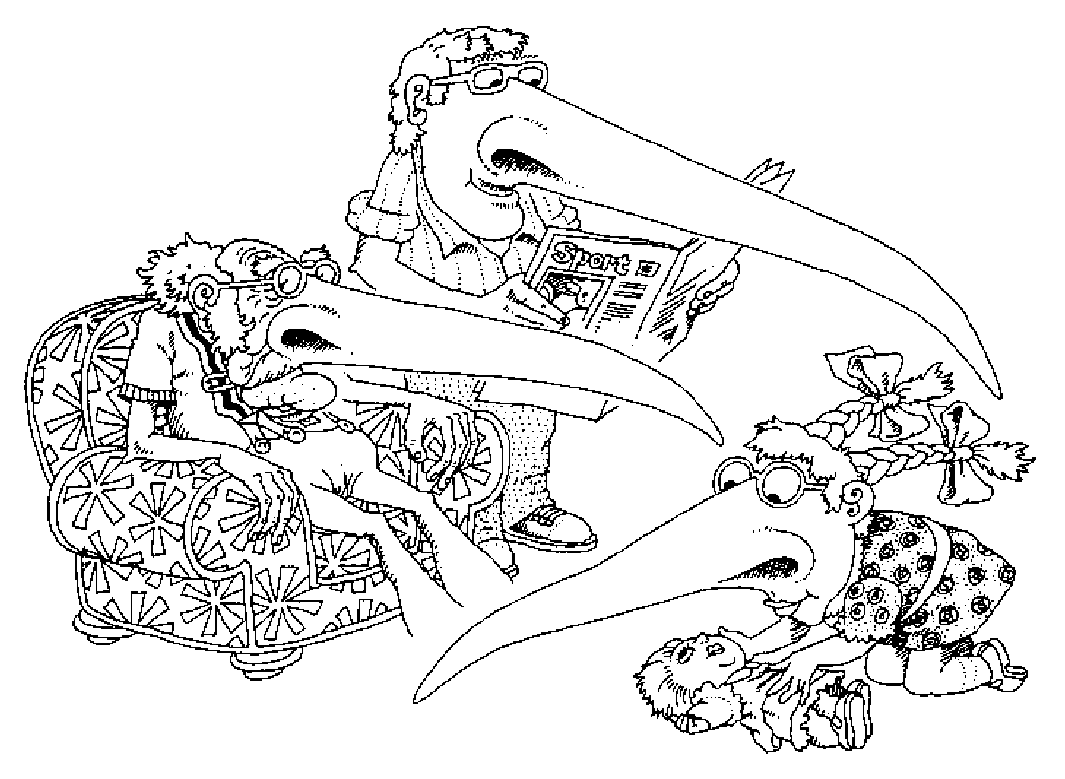
\includegraphics[width=0.7\textwidth]{cartoon6.eps}
        \caption{A subclass may inherit the structure and behaviour
            of its superclass.}
    \end{center}
\end{figure}
\begin{figure}[htb]
    \begin{center}
        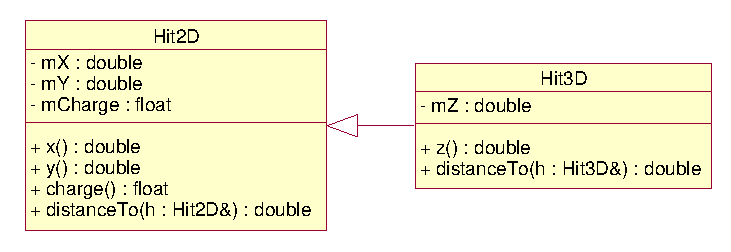
\includegraphics{umlInheritance.eps}
        \caption{Inheritance.}
        \label{fig:umlInheritance}
    \end{center}
\end{figure}

Fig.~\ref{fig:umlInheritance} shows the form of the \emph{inheritance}
relationship.  In this diagram we see that Hit3D is derived from
Hit2D.  If the name of a class would be shown in italics, it would
TrackFitter class and the CalibrartionDB class. This is the \emph{dependency}
relationship. This is often called a \emph{using} relationship.  This
relationship simply means that TrackFitter somehow depends upon
CalibrartionDB. In C++ this almost always results in a \#include:
{\footnotesize
\begin{verbatim}
class Hit3D : public Hit2D {
public:
    double z();
    double distanceTo(Hit3D& h);
private:
    double mZ;
};
\end{verbatim}
}%\footnotesize

\subsection{Aggregation and Association}

The weak form of aggregation is denoted with an open diamond. This
relationship denotes that the aggregate class (the class with the
white diamond touching it) is in some way the "whole", and the other
class in the relationship is somehow "part" of that whole.
Fig.~\ref{fig:umlAggregation} shows an \emph{aggregation}
relationship.
\begin{figure}[htb]
    \begin{center}
        \includegraphics{umlAggregation.eps}
        \caption{Aggregation.}
        \label{fig:umlAggregation}
    \end{center}
\end{figure}
In this case, the Track class contains many Hit instances. In UML the
ends of a relationship are referred to as its "roles''. Notice that
the role at the Hit end of the aggregation is marked with a "$*$".
This indicates that the Track contains many Hit instances.  The
following Listing shows how Fig.~\ref{fig:umlAggregation} might be
implemented in C++ as:

{\footnotesize
\begin{verbatim}
class Track {
public:
    // ...
private:
    vector<Hit*> mHits;
};
\end{verbatim}
}%\footnotesize

There are other forms of containment that do not have whole/part
implications. For example, each \name{Vertex} refers back to its
parent Track. This is not aggregation since it is not reasonable to
consider a parent Track to be part of a child Vertex. We use the
\emph{association} relationship to depict this.

\begin{figure}[htb]
    \begin{center}
        \includegraphics{umlAssociation.eps}
        \caption{Association.}
        \label{fig:umlAssociation}
    \end{center}
\end{figure}

Fig.~\ref{fig:umlAssociation} shows how we draw an association.  An
association is nothing but a line drawn between the participating
classes. In Fig.~\ref{fig:umlAssociation} the association has an
arrowhead to denote that Track does not necessarily know anything
about Vertex. This relationship will almost certainly be implemented
with a pointer of some kind.

What is the difference between an aggregation and an association?
Aggregation denotes whole/part relationships whereas associations do
not. However, there is not likely to be much difference in the way
that the two relationships are implemented.  That is, it would be very
difficult to look at the code and determine whether a particular
relationship ought to be aggregation or association.  Aggregation and
Association both correspond to the \emph{has-by-reference}
relationship.

\subsection{Dependency}

Sometimes the relationship between a two classes is very weak. They
are not implemented with member variables at all. Rather they might be
implemented as member function arguments.

Consider, for example, the fit function of a TrackFitter class.
Suppose that this function takes an argument of type CalibrartionDB
since it requires information from it (e.g. if the magnetic field was
on or off) in order to perform the fit.
\begin{figure}[htb]
    \begin{center}
        \includegraphics{umlDependency.eps}
        \caption{Dependency.}
        \label{fig:umlDependency}
    \end{center}
\end{figure}
Fig.~\ref{fig:umlDependency} shows a dashed arrow between the
TrackFitter class and the CalibrartionDB class. This is the
\emph{dependency} relationship. This is often called a \emph{using}
relationship.  This relationship simply means that TrackFitter somehow
depends upon CalibrartionDB. In C++ this almost always results in a
\#include:

{\footnotesize
\begin{verbatim}
#include "CalibrartionDB.hh"
class TrackFitter {
public:
    // ...
    void fit(CalibrartionDB &db);
private:
    // ...
};
\end{verbatim}
}%\footnotesize

%%%%%%%%%%%%%%%%%%%%%%%%%%%%%%%%%%%%%%%%%%%%%%%%%%%%%%%%%%%%%%%%%%%%
%
% The End
%
%%%%%%%%%%%%%%%%%%%%%%%%%%%%%%%%%%%%%%%%%%%%%%%%%%%%%%%%%%%%%%%%%%%%

\printindex

\end{document}
\bye
% The text following after this line is not included into the text

%
%  Template for reference section
%

%%%%%%%%%%%%%%%%%%%%%%%%%%%%%%%%%%%%%%%%%%%%%%%%%%%%%%%%%%%%%%%%%%%%
%
%    Reference: className
%
%%%%%%%%%%%%%%%%%%%%%%%%%%%%%%%%%%%%%%%%%%%%%%%%%%%%%%%%%%%%%%%%%%%%
\subsection{className}
\index{className|textbf}
\label{sec:className}
\begin{Entry}
\item[Summary]

\item[Synopsis]
    \verb+#include "className.hh"+\\
    \verb+class className;+\\

\item[Description]

\item[Persistence]
    None

\item[Related Classes]

\item[Public\\ Constructors]

\item[Public Member\\ Functions]

\item[Public Member\\ Operators]

\item[Public Functions]

\item[Public Operators]

\item[Examples]
{\footnotesize
\begin{verbatim}
//
//  What the example does
//

\end{verbatim}
}%footnotesize

\end{Entry}
